% $Author$
% $Date$
% $Revision$

% HISTORY:
% Chapter started by Damien C (2009-09-02)

%=================================================================
\ifx\wholebook\relax\else
% --------------------------------------------
% Lulu:
	\documentclass[a4paper,10pt,twoside]{book}
	\usepackage[
		papersize={6.13in,9.21in},
		hmargin={.75in,.75in},
		vmargin={.75in,1in},
		ignoreheadfoot
	]{geometry}
	\input{../common.tex}
	\setboolean{lulu}{true}
% --------------------------------------------
% A4:
%	\documentclass[a4paper,11pt,twoside]{book}
%	\input{../common.tex}
%	\usepackage{a4wide}
% --------------------------------------------
    \graphicspath{{figures/} {../figures/}}
	\begin{document}
\fi
%=================================================================
%\renewcommand{\nnbb}[2]{} % Disable editorial comments
\sloppy
%=================================================================
\chapter{Glamour}
\label{glamour}

Browsers are a crucial instrument to understand complex systems or
models. Each problem domain is accompanied by an abundance of browsers
that are created to help analyze and interpret the underlying
elements. The issue with these browsers is that they are frequently
rewritten from scratch, making them expensive to create and burdensome
to maintain. While many frameworks exist to ease the development of
user interfaces in general, they provide only limited support to
simplifying the creation of browsers.

Glamour is a dedicated framework to describe the navigation flow
of browsers. Thanks to its declarative language, Glamour allows to
quickly define new browsers for their data.

In this chapter we will first detail the creation of some example
browsers to have an overview of the Glamour framework. In a second
part, we will describe Glamour in more details.

\section{Installation and first browser}
\label{sec:inst-first-brows}

To install Glamour on your \pharo{} image execute the following code:

\begin{code}{}
Gofer new
  squeaksource: 'Glamour'; 
  package: 'ConfigurationOfGlamour';
  load.
(Smalltalk at: #ConfigurationOfGlamour)
  perform: #loadDefault.
\end{code}

Now that Glamour is installed, we are going to build a first browser
in order to dive into Glamour's declarative language. What about
building an Apple's Finder-like file browser? This browser is built
using the Miller Columns browsing technique, displaying hierarchical
elements in a series of columns. The principle of such a browser is
that a column always reflects the content of the element selected in
the previous column, the first column-content being chosen on opening.

In our case of implementing a file browser, we want to display a list
of a particular directory's entries (each files and directories) in
the first column and then, depending on the user selection, appending
another column (see \figref{casestudies/file_finder}):

\begin{itemize}
\item if the user selects a directory, the next column will display
  the entries of that particular directory;
\item if the user selects a file, the next column will display the
  content of the file.
\end{itemize}

\begin{figure}
  \begin{center}
    \includegraphics[scale=0.48]{cs_file_finder_final}
    \caption{File finder as a Glamour
      implementation. \label{fig:casestudies/file_finder}}
  \end{center}
\end{figure}

This may look complex at first. However, Glamour provides a very
simple way of describing Miller Columns-based browsers. Glamour calls
that kind of browsers finders, referring to the Apple's Finder found
on Mac OS X. To create such a browser, we are going to use the
\clsind{GLMFinder} class and then tell Glamour that we want elements
to be in a list:

\begin{code}{}
|browser|
browser := GLMFinder new.
browser list
	display: #children.
browser openOn: FSFilesystem onDisk root.
\end{code}

From this small piece of code you get a list of all entries (either
files or directories) found at the root of your file system, each line
representing either a file or a directory. If you click on a
directory, you can see the entries of this directory in the next
column. The filesystem navigation facilities are provided by the
Filesystem framework, thoroughly discussed in \charef{filesystem}.

This code has some problems however. Each line displays the full print
string of the entry and this is probably not what you want. A typical
user would expect only names of each entry. This can easily be done by
customizing the list:

\begin{code}{}
browser list
  display: #children;
  format: #basename.
\end{code}

This way, the message \ct{basename} will be sent to each entry to get its
name. This makes the files and directory much easier to read.

Another problem is that the code does not distinguish between files
and directories. If you click on a file, you will get an error because
the browser will send it the message \ct{children} that it does not
understand. To fix that, we just have to avoid displaying a list of
contained entries if the selected element is a file:

\begin{code}{}
browser list
  when: #isDirectory;
  display: #children;
  format: #basename.
\end{code}

This works well but the user can't distinguish between a line
representing a file or a directory. This can be fixed by, for example,
adding a slash at the end of the file name if it is a directory:

\begin{code}{}
browser list
  when: #isDirectory;
  display: #children;
  format: #basenameWithIndicator.
\end{code}

The last thing we might want to do is to display the contents of the
entry if it is a file. The following gives the final version of the
file browser:

\begin{code}{}
|browser|
browser := GLMFinder new
  variableSizePanes;
  title: 'Find your file';
  yourself.

browser list
  when: #isDirectory;
  display: [:each | [each children sorted]
                       on: Exception
                       do: [Array new]];
  format: #basenameWithIndicator.

browser text
  when: #isFile;
  display: [:entry | [entry readStream contents]
                        on: Exception
                        do: ['Can''t display the content of this file']].
browser openOn: FSFilesystem onDisk root.
\end{code}

This code extends the previous one with variable-sized panes, a title
as well as directory entry sorting, access permission handling and
file content reading. The resulting browser is presented in
\figref{casestudies/file_finder}.

This short
introduction has just presented how to install Glamour and how to use
it to create a simple file browser. 

\section{Tutorial: Implementing a code browser}

The following will present a more complete example as well as detailed
information about the framework.

\subsection{Running example}
\label{sec:tutorial/getting_started}

In the following tutorial we will be creating a simple Smalltalk class
navigator. Such navigators are used in many Smalltalk browsers and
usually consist of four panes, which are abstractly depicted in
figure~\ref{fig:classnavigator_wireframe}.

\begin{figure}[htbp]
\centerline{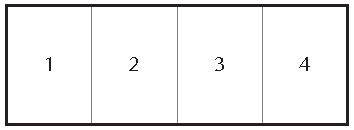
\includegraphics[width=\linewidth]{classnavigator_wireframe.pdf}}
\caption{Wireframe representation of a Smalltalk class navigator.}
\label{fig:classnavigator_wireframe}
\end{figure}

The class navigator functions as follows: Pane~1 shows a list or a
tree of \emph{packages} (containing classes) which make up the
organizational structure of the environment. When a package is
selected, pane~2 shows a list of all classes in the selected
package. When a class is selected, pane~3 shows all \emph{protocols}
(a construct to group methods also known as method categories) and all
methods of the class are shown on pane~4. When a protocol is
selected in pane~3, only the subset of methods that belong to that
protocol are displayed on pane~4.

\subsection{Starting the Browser}

We build the browser iteratively and gradually introduce new
constructs of Glamour. To start with, we simply want to open a new
browser on the list of packages. Because the example is going to
involve more code than the previous file browser, we are going to
implement the code browser in a dedicated class.

The first step is then to create the class with some initial methods:

\begin{code}{}
Object subclass: #PBE2CodeNavigator
  instanceVariableNames: 'browser'
  classVariableNames: ''
  poolDictionaries: ''
  category: 'PBE2-CodeBrowser'

PBE2CodeNavigator class>>open
  ^ self new open

PBE2CodeNavigator>>open
  self buildBrowser.
  browser openOn: self organizer.

PBE2CodeNavigator>>organizer
  ^ RPackageOrganizer default

PBE2CodeNavigator>>buildBrowser
  browser := GLMTabulator new.
\end{code}

Executing \ct{PBE2CodeNavigator open} opens a new browser with the text
``a RPackageOrganizer'' and nothing else. We now extend our browser by
adding a pane to display a list of packages.

\begin{code}{}
PBE2CodeNavigator>>buildBrowser
  browser := GLMTabulator new.
  browser
    column: #packages.

  browser transmit to: #packages; andShow: [:a | self packagesIn: a].

PBE2CodeNavigator>>packagesIn: constructor
  constructor list
    display: [:organizer | organizer packageNames sorted];
    format: #asString
\end{code}

In Glamour browsers are composed in terms of \emph{panes} and the
\emph{flow of data} between them. In our browser we currently have
only one pane displaying packages. The flow of data is specified by
means of \emph{transmissions}. These are triggered when certain
changes occur, such as the change of the selection in a list. To
exemplify this, we extend our browser with a list of classes for the
currently selected package (see \figref{showclasses}).

\begin{code}{}
PBE2CodeNavigator>>buildBrowser
  browser := GLMTabulator new.
  browser
    column: #packages;
    column: #classes.

  browser transmit to: #packages; andShow: [:a | self packagesIn: a].
  browser transmit from: #packages; to: #classes; andShow: [:a | self classesIn: a].

PBE2CodeNavigator>>classesIn: constructor
  constructor list
    display: [:packageName | (self organizer packageNamed: packageName) definedClasses]
\end{code}

\begin{figure}[htbp]
  \centerline{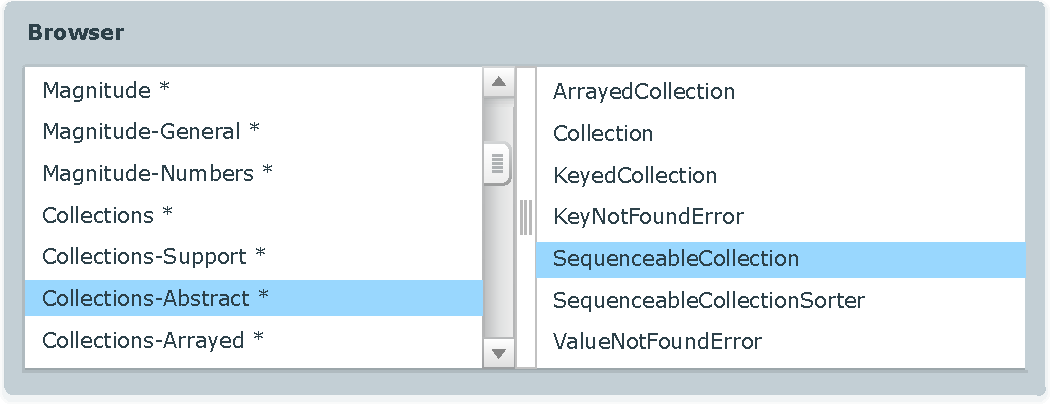
\includegraphics[width=\linewidth]{showclasses.pdf}}
  \caption{Two-pane browser. When a package is selected in the left
    pane, the contained classes are shown on the right pane.}
  \label{fig:showclasses}
\end{figure}

The listing above shows almost all of the core language constructs of
Glamour. Since we want to be able to reference the panes later, we
give them the distinct names ``packages'' and ``classes'' and arrange them
in columns using the \ct{column:} keyword. Similarly, a \ct{row:}
keyword exists with which panes can be organized in rows.

The \ct{transmit:}, \ct{to:} and \ct{from:} keywords create a
\emph{transmission}---a directed connection that defines the flow of
information from one pane to another. In this case, we create a link
from the \emph{packages} pane to the \emph{classes} pane. The
\ct{from:} signifies the \emph{origin} of the transmission and
\ct{to:} the \emph{destination}. If nothing more specific is stated,
Glamour assumes that the origin refers to the \emph{selection} of the
specified pane. We show how to specify other aspects of the origin
pane and how to use multiple origins below.

Finally, the \ct{andShow:} specifies what to display on the destination
pane when the connection is activated or \emph{transmitted}. In our
example, we want to show a list of the classes that are contained in
the selected package.

\ct{display:} simply stores the supplied block within the
presentation. The blocks will only be evaluated later, when the
presentation should be displayed on-screen. If no explicit display
block is specified, Glamour will attempt to display the object in some
generic way. In the case of list presentations, this means that the
\ct{displayString} message will be sent to the object to retrieve a
standard string representation. \ct{format:} can be used to change
this default behavior.

Along with \ct{display:}, it is possible to specify a \ct{when:}
condition to limit the applicability of the connection. By default,
the only condition is that an item is in fact selected, \ie{} that the
display variable argument is not \ct{nil}.

\subsection{Another Presentation}

Up to now, we have been displaying the packages as a list. The
packages in Smalltalk, howerver, are actually organized in a hierarchy
and we have only been looking at the first level of this structure. To
mend this, we replace the list by a tree presentation for packages:

\begin{code}{}
PBE2CodeNavigator>>packagesIn: constructor
  constructor tree
    display: [ :organizer | (self rootPackagesOn: organizer) asSet sorted ];
    children: [ :rootPackage :organizer | (self childrenOf: rootPackage on: organizer) sorted ];
    format: #asString

PBE2CodeNavigator>>classesIn: constructor
  constructor list
    when: [:packageName | self organizer includesPackageNamed: packageName ]
    display: [:packageName | (self organizer packageNamed: packageName) definedClasses];

PBE2CodeNavigator>>childrenOf: rootPackage on: organizer
  ^ organizer packageNames select: [ :name | name beginsWith: rootPackage , '-' ]

PBE2CodeNavigator>>rootPackagesOn: organizer
  ^ organizer packageNames collect: [ :string | string readStream upTo: $- ]
\end{code}

% counter balance the previous $ to avoid a syntax-highlighting bug
% with Emacs

The tree presentation uses a \ct{children:} argument that takes a
selector or a block which specifies how to retrieve the children of a
given item in the tree. Since the children of each package are now
selected by our tree presentation, we have to pass only the roots of
the package hierarchy to the \ct{display:} argument.

At this point, we can also add pane~3 that shows the method categories
as shown in figure~\ref{fig:classnavigator_wireframe}. The listing
below introduces no new elements that we have not already discussed:

\begin{code}{}
PBE2CodeNavigator>>buildBrowser 
  browser := GLMTabulator new.
  browser
    column: #packages;
    column: #classes;
    column: #categories. 

  browser transmit to: #packages; andShow: [:a | self packagesIn: a].
  browser transmit from: #packages; to: #classes; andShow: [:a | self classesIn: a].
  browser transmit from: #classes; to: #categories; andShow: [:a | self categoriesIn: a].

PBE2CodeNavigator>>categoriesIn: constructor
  constructor list
    display:  [:class | class organization categories]  
\end{code}


The browser resulting from the above changes is shown in
figure~\ref{fig:treeandcategories}.

\begin{figure}[htbp]
\centerline{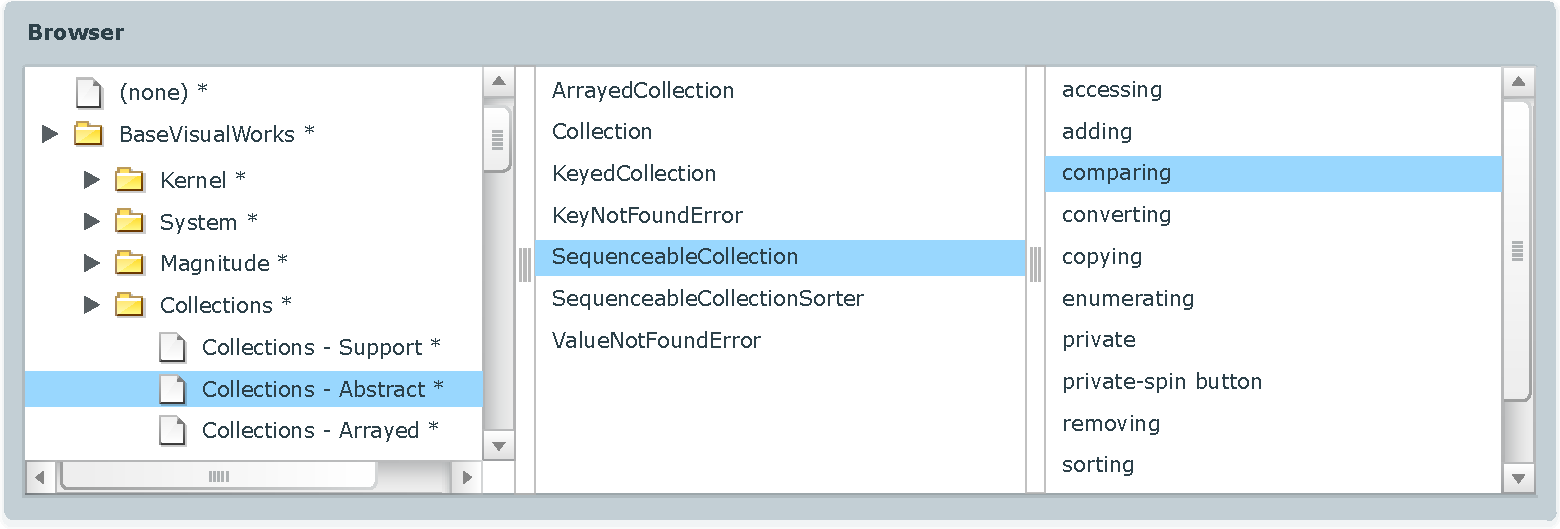
\includegraphics[width=\linewidth]{treeandcategories.pdf}}
\caption{	Improved class navigator including a tree to display the packages and a list of method categories for the selected class.}
\label{fig:treeandcategories}
\end{figure}



%-------------------------------------------------------------------------------
\subsection{Multiple Origins}

The mechanism to show the methods is slightly more complicated. When a
method category is selected we want to show \emph{only} the methods
that belong to that category. If no category is selected, we want to
show \emph{all} methods that belong to the current class.

This leads to our methods pane depending on the selection of two other
panes, the class pane and the category pane. Multiple origins can be
defined using multiple \ct{from:} keywords as shown below.

\begin{code}{}
PBE2CodeNavigator>>buildBrowser
  browser := GLMTabulator new.
  browser
    column: #packages;
    column:  #classes;
    column: #categories;
    column: #methods.

  browser transmit to: #packages; andShow: [:a | self packagesIn: a].
  browser transmit from: #packages; to: #classes; andShow: [:a | self classesIn: a].
  browser transmit from: #classes; to: #categories; andShow: [:a | self categoriesIn: a].
  browser transmit from: #classes; from: #categories; to: #methods; andShow: [:a | self methodsIn: a].

PBE2CodeNavigator>>methodsIn: constructor
  constructor list
    display: [:class :category | (class organization listAtCategoryNamed: category)
                                      sorted].
  constructor list
    when: [:class :category | class notNil and: [category isNil]];
    display: [:class | class selectors sorted];
    allowNil
\end{code}


The listing shows a couple of properties we have not seen
before. First, the multiple origins are reflected in the number of
arguments of the blocks that are used in the \ct{display:} and
\ct{when:} clauses. Secondly, we are using more than one
presentation---Glamour shows all presentations whose conditions match in
the order that they were defined when the corresponding transmission
is fired.

In the first presentation, the condition matches when all arguments
are defined (not nil), this is the default for all presentations. The
second condition matches only when the category is undefined but the
class is not. When a presentation must be displayed even in the
presence of undefined origin, it is necessary to use \ct{allowNil} as
shown. We can therefore omit the category from the display block.

The completed class navigator is displayed in
figure~\ref{fig:codenavigator}.

\begin{figure}[htbp]
\centerline{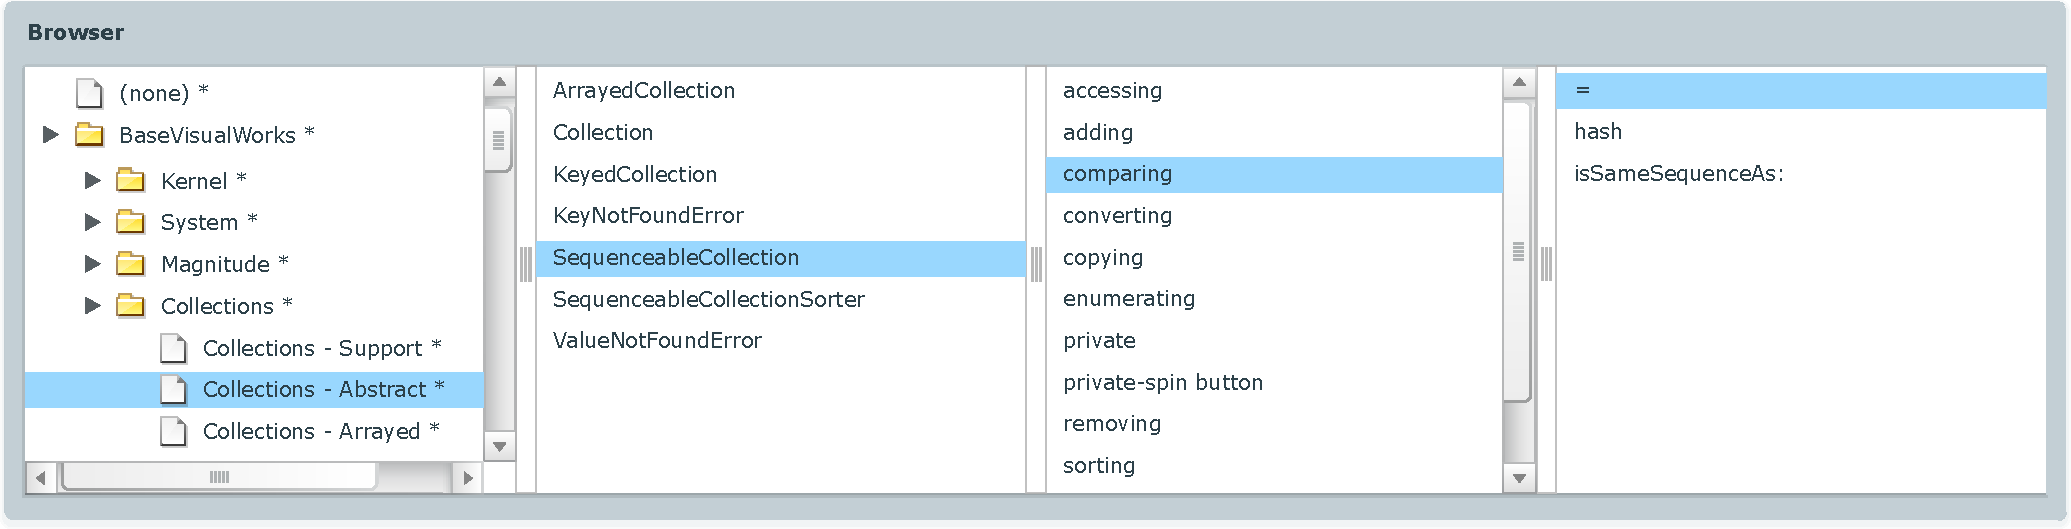
\includegraphics[width=\linewidth]{codenavigator.pdf}}
\caption{Complete code navigator. If no method category is selected, all methods of the class
are displayed. Otherwise, only the methods that belong to that category are shown.}
\label{fig:codenavigator}
\end{figure}


%-------------------------------------------------------------------------------
\subsection{Ports}

When we stated that transmissions connect panes this was not entirely
correct. More precisely, transmissions are connected to properties of
panes called \emph{ports}. Such ports consist of a name and a value
which accommodates a particular aspect of state of the pane or its
contained presentations. If the port is not explicitly specified by
the user, Glamour uses the \emph{selection} port by default. As a
result, the following two statements are equivalent:

\begin{code}{}
browser transmit from: #packages; to: #classes; andShow: [:a | ...].
browser transmit from: #packages port: #selection; to: #classes; andShow: [:a | ...].
\end{code}

\dc{It is currently not clear what are the available ports for each
  presentation. It looks like hover does not exist anymore}

Other ports exist and may be used depending on the presentation. For
example, the list presentation also populates the \emph{hover} port
when the user hovers over an item over a list and a text presentation
updates the \emph{text} port to reflect its contents as a user types
within it. For a full reference, see the documentation of the
presentations being used.


%-------------------------------------------------------------------------------
\subsection{Reusing Browsers}
\label{sec:tutorial/reusing-browsers}

One of the strengths of Glamour lies in the ability to use browsers in
place of primitive presentations such as lists and trees. This allows
us to reuse browsers and nest them within each other.

In the next example we want to create a class \emph{editor} as shown
in figure~\ref{fig:classbrowser_wireframe}. Panes 1 through 4 are
equivalent to those described previously. Pane~5 shows the source code
of the method that is currently selected in pane~4.

\begin{figure}[htbp]
\centerline{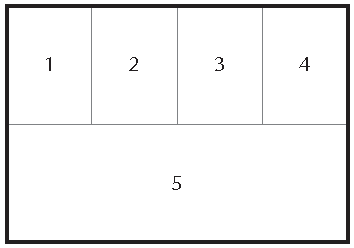
\includegraphics[width=\linewidth]{classbrowser_wireframe.pdf}}
\caption{Wireframe representation of a Smalltalk class editor.}
\label{fig:classbrowser_wireframe}
\end{figure}

For the sake of the example, we will create this editor in a new class
called \ct{PBE2CodeEditor}. This editor will delegate the presentation
of panes 1 through 4 to the previously implemented
\ct{PBE2CodeNavigator}. To achieve this, we first have to make the
existing navigator return the constructed browser.

\begin{code}{}
PBE2CodeNavigator>>buildBrowser
  [...]
  ^ browswer
\end{code}

We can then reuse the navigator in the new editor browser as shown
below.

\begin{code}{}
Object subclass: #PBE2CodeEditor
	instanceVariableNames: 'browser'
	classVariableNames: ''
	poolDictionaries: ''
	category: 'PBE2-CodeBrowser'.

PBE2CodeEditor class>>open
  ^ self new open

PBE2CodeEditor>>open
  self buildBrowser.
  browser openOn:  self  organizer

PBE2CodeEditor>>organizer 
  ^ RPackageOrganizer default

PBE2CodeEditor>>buildBrowser 
  browser := GLMTabulator new.
  browser 
    row: #navigator;
    row: #source.
    
  browser transmit to: #navigator; andShow:  [:a | self navigatorIn: a ]. 

PBE2CodeEditor>>navigatorIn:  constructor
  constructor  custom:  (PBE2CodeNavigator new buildBrowser)
\end{code}


The listing shows how the browser is used exactly like we would use a
list or other type of presentation. In fact, browsers are a type of
presentation.

When evaluating the code \ct{PBE2CodeEditor open}, a new browser is
opened that shows the navigator embedded in the top pane and an empty
pane at the bottom. No source code will be displayed because we have
not yet created any connections between the panes. To get to the
source, we need both the name of the selected method as well as the
class in which it is defined. Since this information is defined only
within the navigator browser, we must first export it to the outside
world by using the \ct{sendToOutside:from:} message. For this we
append the following lines to \ct{codeNavigator}:

\begin{code}{}
PBE2CodeNavigator>>buildBrowser
  [...]
  browser transmit from: #classes; toOutsidePort:  #selectedClass. 
  browser transmit from: #methods; toOutsidePort:  #selectedMethod.
  
  ^ browser
\end{code}

This will send the selection within classes and methods to the
\emph{selectedClass} and \emph{selectedMethod} ports of the containing
pane. Alternatively, we could have added these lines to the
\ct{navigatorIn:} method in the code editor---it makes no difference
to Glamour.

\begin{code}{}
PBE2CodeEditor>>navigatorIn: constructor

  "Alternative way of adding outside ports. There is no need to use this
   code and the previous one simultaneously."

  | navigator |
  navigator := PBE2CodeNavigator new buildBrowser
          sendToOutside: #selectedClass from: #classes -> #selection;
          sendToOutside: #selectedMethod from: #methods -> #selection;
          yourself.
  
  constructor custom: navigator
\end{code}

However, we consider it sensible to clearly define the interface on
the side of the code \emph{navigator} rather than within the code
editor in order to promote the reuse of this interface as well.

Note that a message for achieving the reverse---importing a port from
the outside pane and storing its value on one of the browser's panes
also exists and requires the use of \ct{fromOutsidePort:} and \ct{to:}.

We extend our code editor example as follows:

\begin{code}{}
PBE2CodeEditor>>buildBrowser 
	browser := GLMTabulator new.
	browser 
		row: #navigator;
		row: #source.
		
	browser transmit to: #navigator; andShow:  [:a | self navigatorIn: a ]. 
	browser transmit
		from:  #navigator port: #selectedClass;
		from: #navigator port: #selectedMethod;
		to: #source;
		andShow:  [:a | self sourceIn: a].

PBE2CodeEditor>>sourceIn: constructor
	constructor text
		display: [:class :method | class sourceCodeAt: method] 
\end{code}


We can now view the source code of any selected method and have
created a modular browser by reusing the class navigator that we had
already written earlier. The composed browser described by the listing
is shown in figure~\ref{fig:composed-browser}.

\begin{figure}[htbp]
\centerline{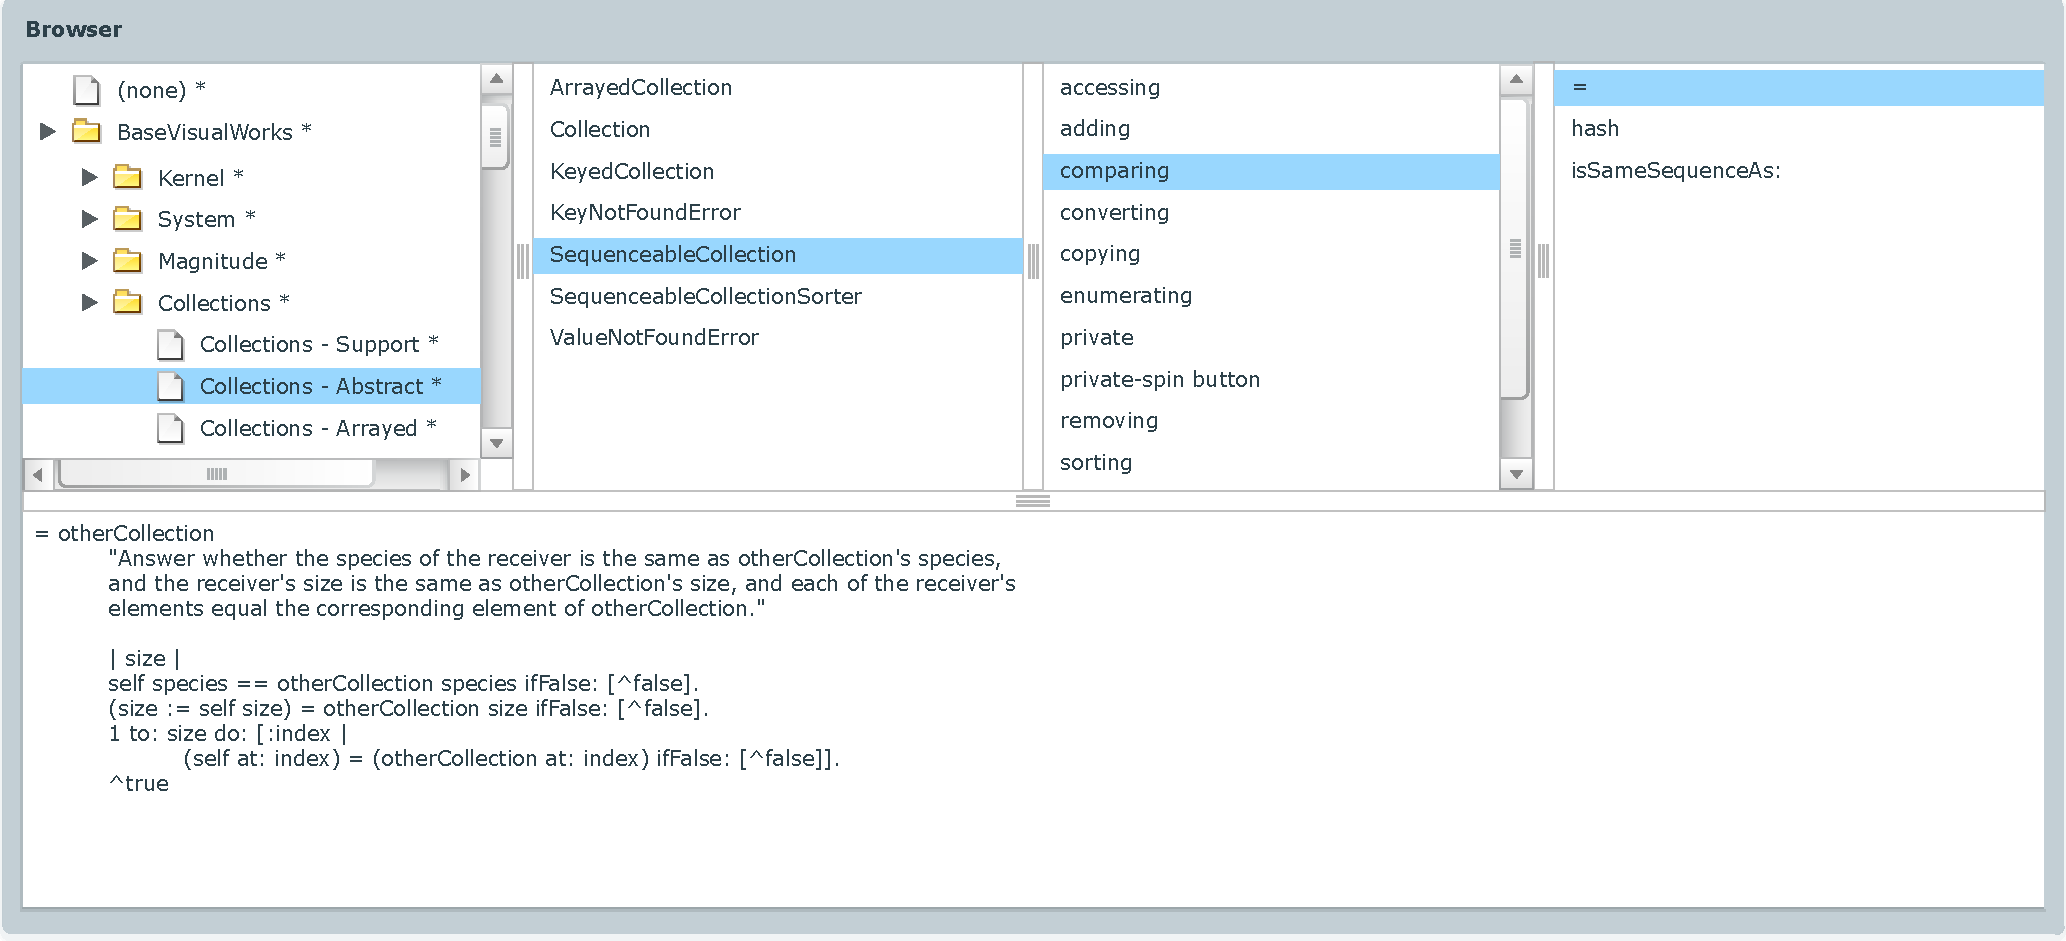
\includegraphics[width=\linewidth]{classbrowser.pdf}}
\caption{Composed browser that reuses the previously described class navigator to show the source of a selected method.}
\label{fig:composed-browser}
\end{figure}

%-------------------------------------------------------------------------------
\subsection{Actions}
\label{sec:tutorial/actions}

Browsers generally rely on \emph{actions}---first-class behavioral objects that are executed when a keyboard shortcut is pressed or when an entry in a context menu is clicked. Glamour supports such actions through the \ct{act:on:} message sent to a presentation:

\begin{code}{}
PBE2CodeEditor>>sourceIn: constructor
  constructor text
    display: [:class :method | class sourceCodeAt: method ];
    act: [:presentation :class :method | class compile: presentation text] on: $s.
\end{code}

% a $ for balance

The argument passed to \ct{on:} is a character that specifies the
keyboard shortcut that should be used to trigger the action when the
corresponding presentation has the focus. Whether the character needs
to be combined with a meta-key---such as command, control or alt---is
platform specific and need not be specified. The \ct{act:} block
provides the corresponding presentation as its first argument which
can be used to poll its various properties such as the contained text
or the current selection. The other arguments to the block are the
incoming origins as defined by \ct{from:} and are equivalent to the
arguments of \ct{display:} and \ct{when:}.

Actions can also be displayed as context menus. For this purpose,
Glamour provides the messages \ct{act:on:entitled:} and
\ct{act:entitled:} where the last argument is a string that should be
displayed as the entry in the menu. For example, the following snippet
extends the above example to provide a context menu entry to ``save''
the current method back to the class:
\begin{code}{}
...
  act: [:presentation :class :method | class compile: presentation text]
  on: $s.
  entitled: 'Save'
\end{code}

%$

%-------------------------------------------------------------------------------
\subsection{Multiple Presentations}

Frequently, developers wish to provide more than one presentation of a
specific object. In our code browser for example, we may wish to show
the classes not only as a list but as a visualization of their
\emph{system complexity} as well. Glamour includes support to display
and interact with visualizations created using the \emph{Mondrian
  visualization engine}. To add a second presentation, we simply
define it in the \ct{using:} block as well:

\begin{code}{}
PBE2CodeNavigator>>classesIn: constructor
  constructor list
    when: [:packageName | self organizer includesPackageNamed: packageName ];
    display: [:packageName | (self organizer packageNamed: packageName)
                    definedClasses];
    title: 'Class list'.

  constructor mondrian 
    when: [:packageName | self organizer includesPackageNamed: packageName];
    painting: [ :view :packageName | 
          view nodes: (self organizer packageNamed:  packageName)  
                             definedClasses.
          view edgesFrom:  #superclass.
          view treeLayout];
    title: 'Hierarchy' 
\end{code}

Glamour distinguishes multiple presentations on the same pane with the
help of a tab layout. The appearance of the Mondrian presentation as
embedded in the code editor is shown in
figure~\ref{fig:mondrian-presentation}. The clause \ct{title:} sets
the name of the tab used to render the presentation.

\begin{figure}[htbp]
\centerline{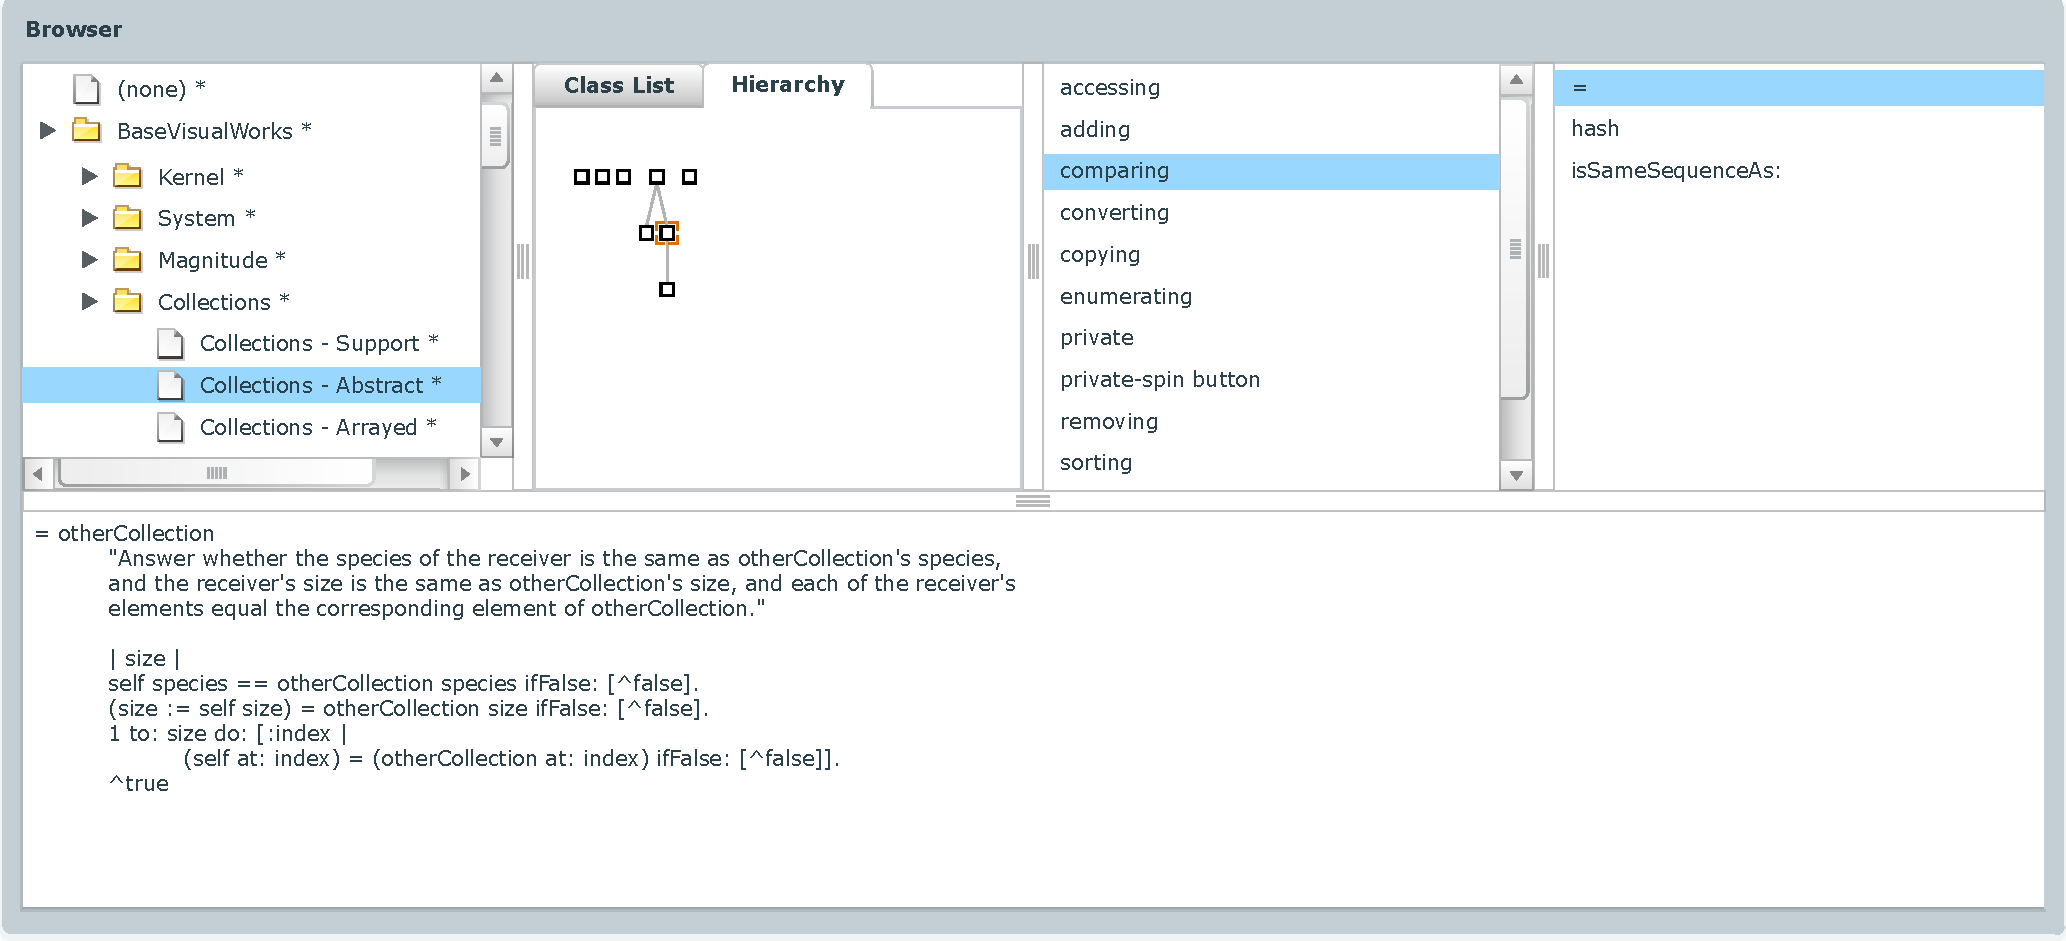
\includegraphics[width=\linewidth]{mondrian-presentation.pdf}}
\caption{Code editor sporting a Mondrian presentation in addition to a simple class list.}
\label{fig:mondrian-presentation}
\end{figure}


%-------------------------------------------------------------------------------
\subsection{Other Browsers}

Up to now in the tutorial, we have only used the \ct{GLMTabulator}
which is named after its ability to generate custom layouts using the
aforementioned \ct{row:} and \ct{column:} keywords. Additional
browsers are provided or can be written by the user. Browser
implementations can be subdivided into two categories: browsers that
have \emph{explicit panes}, \ie{}, they are declared explicitly by the
user---and browsers that have \emph{implicit panes}.

The \ct{GLMTabulator} is an example of a browser that uses explicit
panes. With implicit browsers, we do not declare the panes directly
but the browser creates them and the connections between them
internally. An example of such a browser is the \ct{Finder}, which has
been discussed in \secref{sec:inst-first-brows}. Since the panes are
created for us, we need not use the \ct{from:to:} keywords but can
simply specify our presentations:

\begin{code}{}
browser := GLMFinder new.

browser list
  display: [:class | class subclasses].

browser openOn: Collection
\end{code}

The listing above creates a browser (shown in figure~\ref{fig:finder})
and opens to show a list of subclasses of \emph{Collection}. Upon
selecting an item from the list, the browser expands to the right to
show the subclasses of the selected item. This can continue
indefinitely as long as something to select remains.

\begin{figure}[htbp]
\centerline{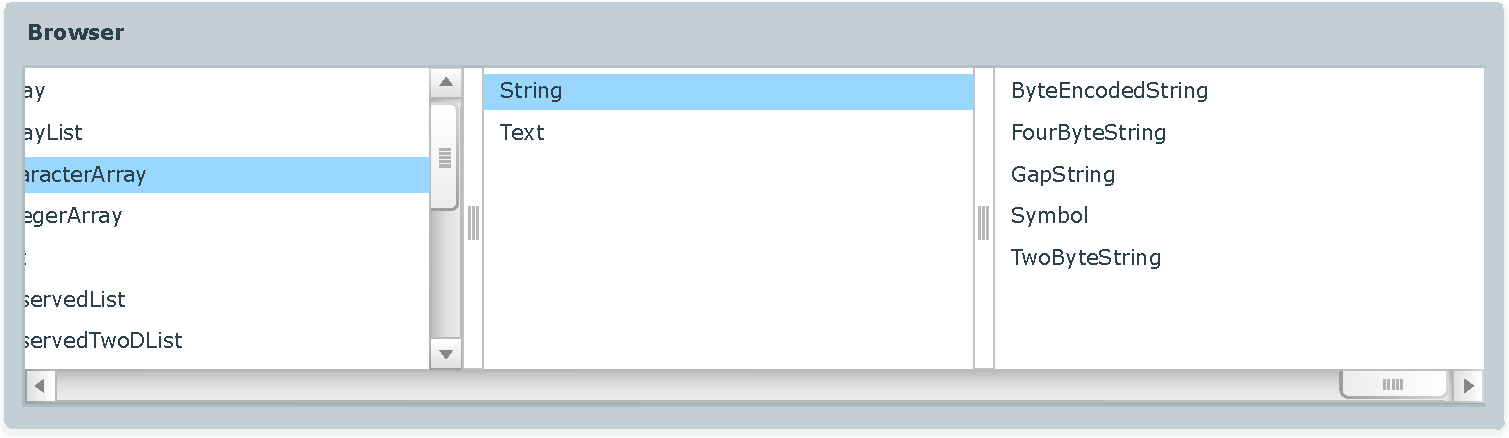
\includegraphics[width=\linewidth]{finder.pdf}}
\caption{Subclass navigator using Miller Columns style browsing.}
\label{fig:finder}
\end{figure}

To discover other kinds of browsers, explore the hierarchy of the
\ct{GLMBrowser} class.

%-------------------------------------------------------------------------------
\subsection{Tutorial Conclusion}

This concludes our tutorial of Glamour. Please note that this tutorial
is not meant to give an exhaustive overview of Glamour, but is merely
intended to introduce the reader to the usage and to our intent for
our approach. For a more extensive view of Glamour, its concepts and
implementation, the Moose
book\footnote{\url{http://www.themoosebook.org/book}} has a dedicated
chapter dedicated.

%=============================================================
\ifx\wholebook\relax\else
   \bibliographystyle{jurabib}
   \nobibliography{scg}
   \end{document}
\fi
%=============================================================




%-----------------------------------------------------------------

%%% Local Variables:
%%% coding: utf-8
%%% mode: latex
%%% TeX-master: t
%%% TeX-PDF-mode: t
%%% ispell-local-dictionary: "english"
%%% End: